\documentclass[helvetica, 10pt]{article}

% If you're new to LaTeX, here's some short tutorials:
% https://www.overleaf.com/learn/latex/Learn_LaTeX_in_30_minutes
% https://en.wikibooks.org/wiki/LaTeX/Basics

% Formatting
\usepackage{blindtext}
\usepackage[T1]{fontenc}
\usepackage[utf8]{inputenc}
\usepackage[margin=1in]{geometry}

% Math
% https://www.overleaf.com/learn/latex/Mathematical_expressions
\usepackage{amsmath, amsfonts, amssymb, mathtools}

% Images
% https://www.overleaf.com/learn/latex/Inserting_Images
\usepackage{graphicx, float}

% Algorithms
% https://www.overleaf.com/learn/latex/algorithms
% https://en.wikibooks.org/wiki/LaTeX/Algorithms
\usepackage[ruled,vlined]{algorithm2e}
\usepackage{algorithmic}

% Code syntax highlighting
% https://www.overleaf.com/learn/latex/Code_Highlighting_with_minted
\usepackage{minted}
\usemintedstyle{borland}


% ====================== TITLE =========================================
\title{Artificial intelligence - Project 1 \\ - Search problems - }

% introduceti numele autorului aici
\author{George Botis & Daria Francioli}
\date{7/11/2022}

\begin{document}

\maketitle
\thispagestyle{empty}

\section{Introducere}

Scopul acestui proiect este acela de a implementa alți algoritmi de căutare pentru a-l ajuta pe Mr. Pacman să găsească mâncarea în cel mai scurt timp. Vom face și o comparație între cei 2 algoritmi noi (Un algoritm bidirecțional și Weighted A*) și cei 4 deja reprezentați în laboratoarele anterioare ( BFS, DFS, A* și UCS) . \newline


\subsection{Definirea problemei și soluționarea acesteia}

Prin compararea mai multor algoritmi de căutare vrem să rezolvăm problema găsirii drumului spre mâncare în cel mai scurt timp. 
\newline
\newline
Adițional am mai creat-o și pe Miss Pacman, jucându-ne cu grafica Pacmanului original, adăugând o fundiță, gene și ochi albaștrii ce se deplasează odată cu Miss Pacman. 

\subsection{Algoritmii folosiți}

\begin{enumerate}
  \item Bidirectional Algorithm
  \item Weighted A* 
  \item BFS, DFS, UCS, A*
\end{enumerate}
\newline
Algoritmii de căutare DFS, BFS, UCS și cel bidirecțional sunt algoritmi neinformați(constă în explorarea alternativelor, fără a utiliza informații specifice despre problemă).
\newline
\newline
Algoritmii de căutare A* și Weighted A* sunt algoritmi informați(euristică-încearcă alegerea „inteligentă” a nodurilor care trebuie expandate).
\newline

\begin{figure}[h]
    \centering
    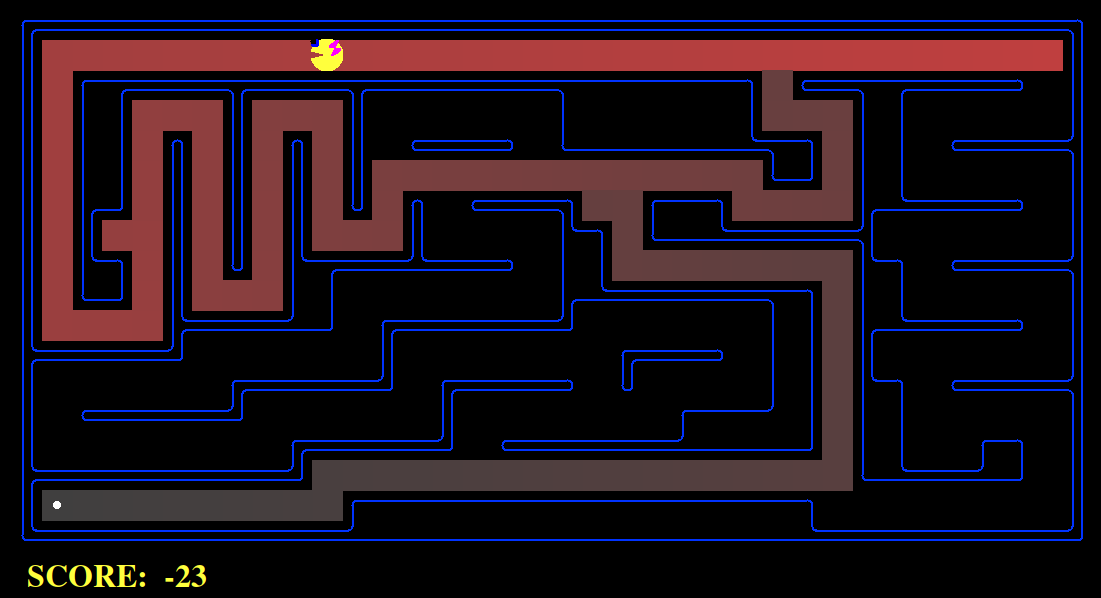
\includegraphics[width=16cm]{text/images/pic1.png}\\
    \caption{Medium Maze Miss Pacman}
\end{figure}




\section{Implementare}
% enuntul intrebarii
În această secțiune vom prezenta implementarea fiecărui algoritm.
\newline

% ============================================= BFS ============================================= 

\subsection{Breadth First Search (BFS)}
Algoritmul BFS este un algoritm de căutare utilizat în grafuri și arbori, de asemenea poate fi folosit pentru 
Frontiera BFS este bazată pe FIFO (primul intrat, primul ieșit) și extinde succesorii în ordinea în care au fost adăugați.
Se merge pe lățime prin nodurile vecine ale punctului în care ne aflăm.\newline

\textbf{Cod:}
% a se completa fisierul code/bfs.py
\inputminted[linenos]{python}{code/02_bfs.py}


\textbf{Explicație:}
\begin{itemize}
    \setlength\itemsep{0em}
    \item funcția problem va returna o solutie sau fail, se va stoca succesorii într-o coadă, verifică dacă fiecare nod a fost vizitat, îi dă push către visited pentru a evita verificarea de mai multe ori a unui nod deja vizitat, si se verifică daca am ajuns la goalState- dacă nu, de va da expand copiilor după algoritm.

\end{itemize}


\textbf{Comandă:}
\begin{itemize}
    \setlength\itemsep{0em}
    \item python pacman.py -l mediumMaze -p SearchAgent -a fn=bfs
        
\end{itemize}

\subsubsection{Întrebări}

\textbf{Q1:} Soluția găsită este optimă? Explicați răspunsul.
\newline
\textbf{A1:} BFS este optim numai dacă costul tuturor arcelor din graficul spațiului de stare este același.
\newline
\newline
\textbf{Q2:} Run autograder \textit{python autograder.py} and write the points for Question 2.
\newline
\textbf{A2:} Question q2: 3/3
\newline
\vspace{0.75cm}
\pagebreak

% ============================================= DFS ============================================= 

\subsection{Depth First Search (DFS)}
DFS caută mai întâi cel mai adânc nod din arborele de căutare.\newline

\textbf{Cod:}
% a se completa fisierul code/dfs.py
\inputminted[linenos]{python}{code/01_dfs.py}


\textbf{Explicație:}
\begin{itemize}
    \setlength\itemsep{0em}
    \item Frontiera DFS este bazată pe LIFO (ultimul intrat, primul ieșit) și extinde succesorii în ordinea în care au fost adăugați. Se merge pe adâncime prin nodurile vecine ale vecinilo punctului în care ne aflăm până când ajungem la starea GOAL.
    Odată ce un nod este complet extins, acesta este popped din stivă.

\end{itemize}


\textbf{Comandă:}
\begin{itemize}
    \setlength\itemsep{0em}
    \item python pacman.py -l mediumMaze -p SearchAgent -a fn=dfs
        
\end{itemize}

\subsubsection{Întrebări}

\textbf{Q1:} Soluția găsită este optimă? Explicați răspunsul.
\newline
\textbf{A1:} DFS nu este optim. Găsește doar soluția cea mai din stânga în arborele de căutare, indiferent de adâncimea sau costul nodului.
\newline
\newline
\textbf{Q2:} Run autograder \textit{python autograder.py} and write the points for Question 2.
\newline
\textbf{A2:} Question q2: 3/3
\newline
\vspace{0.75cm}
\pagebreak


% ============================================= A*  ============================================= 
\subsection{A* search  algorithm}
% enuntul intrebarii
Costul total al unui nod nu trebuie să fie mai mic decât suma dintre cost(distanță start+distanță curentă) și euristica folosită. \newline

\textbf{Cod:}
% a se completa fisierul code/4_a_star.py
\begin{listing}[h]
    \inputminted[linenos]{python}{code/04_a_star.py}
\end{listing}


\textbf{Explicație:}
\begin{itemize}
    \setlength\itemsep{0em}
    \item Euristica ia două argumente: o stare în problema de căutare (argumentul principal) și problema în sine (pentru informații de referință). Folosim o coadă de priorități, care este dată de cost și euristică. Funcția folosită este f(n)= g(n)+h(n)(g=cost, h=euristica) și dacă următoarea stare în care ne-am afla este următorul nod, atunci expandăm nodul stării și actualizăm starea următoare cu locația porții destinație. 

\end{itemize}


\textbf{Comandă:}
\begin{itemize}
    \setlength\itemsep{0em}
    \item  -l tinyMaze -p SearchAgent -a fn=aStar
        
\end{itemize}

\subsubsection{Questions}
This sub-section is dedicated to the additional questions that come along with the exercise. Please answer to the following questions:\newline


\textbf{Q1:} A* și UCS au aceeași soluție sau sunt diferite?

\textbf{A1:} Este asemănător cu UCS, dar alege starea următoare.\newline

\textbf{Q2:} Run autograder \textit{python autograder.py} and write the points for Question 4 (min 3 points).


\textbf{A4:}  Question q2: 3/3

\vspace{0.75cm}
\pagebreak

% ============================================= UCS ============================================= 
\subsection{Uniform-Cost Search (UCS)}
% enuntul intrebarii
În loc să extindă cel mai puțin adânc nod, cum ar fi BFS, extinde nodul n cu calea cu cel mai mic cost g(n). Schimbând funcția de cost, putem încuraja Pacman să găsească căi diferite. De exemplu, costul pentru pașii periculoși în zonele pline de fantome este mai mare.\newline

\textit{"In search.py,  implement  \textbf{Uniform-cost graph search} algorithm  in \textit{uniformCostSearchfunction}"}

\textbf{Cod:}
% a se completa fisierul code/ucs.py
\inputminted[linenos]{python}{code/03_ucs.py}

\textbf{Explicație:}
\begin{itemize}
    \setlength\itemsep{0em}
    \item Aplică test Goal unui nod odată ce acesta este selectat pentru extindere,nu ca atunci când este generat prima dată (ca în cazul BFS și DFS). Acest lucru se datorează faptului că primul nod de goal care este generat poate fi pe o cale suboptimă. Include, de asemenea, un test pentru a verifica dacă a fost întâlnită o stare de goal mai bună.

\end{itemize}

\textbf{Comenzi:}
\begin{itemize}
    \setlength\itemsep{0em}
    \item python pacman.py -l mediumMaze -p SearchAgent -a fn=ucs
        
\end{itemize}

\subsubsection{Întrebări}

\textbf{Q1:} Comparați rezultatele cu cele obținute cu DFS. Sunt soluțiile diferite? Explicați răspunsul.
\newline
\textbf{A1:} UCS este similar cu DFS, dar are o coadă de prioritate pentru stocarea succesorilor+ fiecare cost este atașat.
\newline
\newline
\textbf{Q2:} Run autograder \textit{python autograder.py} and write the points for Question 2.
\newline
\textbf{A2:} Question q2: 3/3
\newline
\vspace{0.75cm}
\pagebreak

% ============================================= Bidirectional Search  ============================================= 

\subsection{Bidirectional Search}
Algoritmul abordeaza problema pornind atat de la punctul de start cat si de la punctul target. Ideea generala este de a determina un path de la start la finish si un alt path de la finish la start pentru a determina locul in care aceste path-uri se intalnesc.\newline

\textbf{Cod:}
% a se completa fisierul code/bi.py
\inputminted[linenos]{python}{code/05_bi.py}

\pagebreak
\textbf{Explicație:}
\begin{itemize}
    \setlength\itemsep{0em}
    \item La prima instanta a unui punct de contact (daca exista) algoritmul va creea path-ul final care consta intr-o combinatie a celor 2 path-uri initiale: Prima parte de la start pana la punctul de contact si a doua parte de la finish la punctul de contact.
In teorie, algoritmul este mai rapid decat un BFS sau un DFS clasic. Daca complexitatea unui DFS este O(b^d), complexitatea bidirectionalului este O(b^(d/2) +b^(d/2)) care este mult mai mic decat O(b^d).

\end{itemize}


\textbf{Comandă:}
\begin{itemize}
    \setlength\itemsep{0em}
    \item python pacman.py -l mediumMaze -p SearchAgent -a fn=bi
        
\end{itemize}

\subsubsection{Întrebări}

\textbf{Q1:} Soluția găsită este optimă? Explicați răspunsul.
\newline
\textbf{A1:} BFS este optim numai dacă costul tuturor arcelor din graficul spațiului de stare este același.
\newline
\newline
\textbf{Q2:} Run autograder \textit{python autograder.py} and write the points for Question 2.
\newline
\textbf{A2:} Question q2: 3/3
\newline
\vspace{0.75cm}
\pagebreak


% ============================================= Weighted A* ============================================= 

\subsection{Weighted A*}
După cum se poate observa, există o diferență între acest algoritm și cel clasic: Epsilon. Fiind un algoritm informat, are o euristică= Euristica Euclidiană.\newline
Dacă epsilon < 1, epsilon merge catre 0, iar algoritmul va căuta calea cu cel mai redus cost.
Dacă epsilon = 0, algoritmul se comportă la fel ca Uniform Cost Search.
Dacă epsilon = 1, algoritmul se comportă la fel ca A Star.
Dacă epsilon > 1, epsilon merge catre infinit, iar algoritmul va deveni unul de tip greedy.\newline

\textbf{Cod:}
% a se completa fisierul code/wastar.py
\inputminted[linenos]{python}{code/06_wastar.py}


\textbf{Explicație:}
\begin{itemize}
    \setlength\itemsep{0em}
    \item În funcție de datele de intrare și soluția pe care vrem să îl atingem, alegem epsilon. 

\end{itemize}


\textbf{Comandă:}
\begin{itemize}
    \setlength\itemsep{0em}
    \item python pacman.py -l bigMaze -p SearchAgent fn=wastar
        
\end{itemize}

\subsubsection{Întrebări}

\textbf{Q1:} Soluția găsită este optimă? Explicați răspunsul.
\newline
\textbf{A1:} Weighted A* este mai optim decât cel clasic datorită epsilonului cu care configurăm algoritmul.
\vspace{0.75cm}
\pagebreak

\section{Grafica pentru Miss Pacman}
% enuntul intrebarii
În această secțiune vom prezenta implementarea grafică a Miss Pacman.
\newline

\subsection{Draw Miss Pacman}
Pentru a o desena pe Miss Pacman am folosit modelul de grafică pentru fantome, dar în loc de două cercuri pentru doi ochi, va avea 2 cercuri pentru unul, si vor fi unul peste altul, de dimensiuni diferite. De asemenea Miss Pacman are o fundă mov care nu putea lipsi din designul nostru. \newline

\textbf{Cod din GraphicDesign:}
% a se completa fisierul code/mspacman.py
\inputminted[linenos]{python}{code/mspacman.py}

\begin{figure}[h]
    \centering
    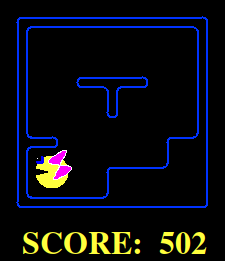
\includegraphics[width=6cm]{text/images/miss pacman.png}\\
    \caption{Miss Pacman}
\end{figure}


\vspace{0.75cm}
\pagebreak

\include{text/4_Testare și Comparare}
\section{Conluzii}
Prin intermediul acestui proiect, noi am reușit să descoperim bazele și sintaxele limbajului python: definirea variabilelor, apelul unor funcții sau metode, instanțierea de obiecte și transmiterea parametriilor de la o funcție sau metodă la alta. 

De asemenea ne-am amintit algoritmii de căutare și utilozarea acestora în grafuri, arbori, printr-un mod mai practic și creativ. Am reușit să le testam astfel optimitatea și să-l alegem pe cel câștigător pentru Pacman.
Pacmanul nostru și-a atins scopul: a ajuns la mâncare.\newline\newline

\begin{figure}[h]
    \centering
    
\includegraphics[width5cm]{text/images/pacman.png}\\

\end{figure}



\end{document}